\chapter{Introduction to Knox}\label{introduction_to_knox}
\textit{The following sections have been written in collaboration with other Knox project groups.}

Knox is a large-scale collaborative project offered at the 5th semester of the Software study program at Aalborg University in the fall of 2021. It is a multi-project in the sense that eight groups are to work together to facilitate a noticeable increment compared to the work of last year's 5th semester students, who initiated Knox. In other words - besides being a multi-group project, Knox is also a cross-semester project with each year's students handing over their contribution to future 5th semester students.\\

Knox is an acronym of The Knowledge Toolbox, and as the name implies it is a knowledge engineering toolbox. The vision for Knox is a flexible knowledge engineering toolbox with components that can be combined to solve bigger problems. Currently, the project is focused on processing documents with \textit{Nordjyske Mediehus} and \textit{Grundfos} as collaborators who supply large amounts of documents to hopefully be turned into knowledge through Knox.\\

With this semester, Knox is going into its second year of development, during which the role of product owner is carried out by a student from the previous year of Knox development. Project handover is done with the help of the product owner. The status of Knox at handover is that a foundation has been built by last year's students.
However, the search engine, Knox's most basic component, is not currently functional. Getting the search engine to a functional state is an important part of this year's development.\\

For the second year of development, there exist two primary stages.
The first stage is to get the pipeline with search engine functionality up and running as a minimum viable product (MVP). The MVP will be decided by the groups together with the Product Owner (PO). The second stage is for the groups to individually extend their layer's functionality. This stage should hopefully bring the Knox pipeline beyond the MVP and give extended functionality to the toolbox.\\

To give a better idea of the Knox project as a whole, the pipeline will now be presented and explained. 

\section{The Knox pipeline}\label{the_knox_pipeline}
\textit{The following section has been written in collaboration with other Knox project groups.}


The Knox pipeline is made up of four separate layers, which each is responsible for providing components and functionality to the system.
 Additionally, three of the layers are separated between working with either \textit{Nordjyske Mediehus} or \textit{Grundfos}.
  A figure illustrating the entire pipeline can be seen in figure \ref{fig:pipeline}.

\begin{figure}[h]
    \centering
    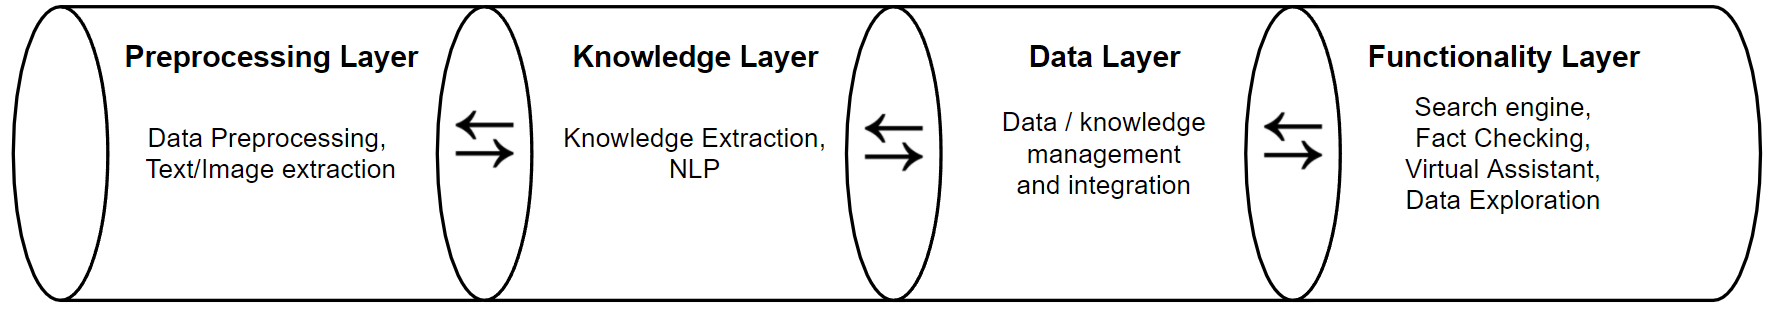
\includegraphics[width=1\textwidth]{Images/Pipeline.PNG}
    \caption{Illustration of the Knox pipeline\label{fig:pipeline}.}
\end{figure}

Last year, a User Interface (UI) layer was introduced. This year, the responsibility of creating UI elements have been split among all groups, who provide interface for their own systems.

\subsubsection{Preprocessing Layer}
The preprocessing layer is responsible for extracting data from \textit{Nordjyske Mediehus} articles and \textit{Grundfos} manuals. Many of these documents are photo scans of old articles, which means that both font, layout, and quality varies from document to document. For this reason, it is necessary to convert many of the documents to a standard format, before it is possible to extract any data. The result should allow all data from \textit{Nordjyske Mediehus} and \textit{Grundfos} to be extracted. 

\subsubsection{Knowledge layer}
The knowledge layer is used to process the data extracted by the preprocessing layer. Methods like Natural Language Processing (NLP) algorithms should be applied to extract knowledge, word count should be tallied and sent to the database, or the text should be annotated to extract entities and their relations, enabling a knowledge graph to be constructed.

\subsubsection{Data layer}\label{databaseResponsibility}
The data layer is responsible for handling the flow of data between the knowledge layer and the functionality layer in the \knox{} pipeline.
New data must be stored on the servers, and it must be accessible to the components that need it. 
This requires close cooperation with the other layers in the pipeline.


As multiple components in the \knox{} system both provide and require access to data, there needs to be a streamlined process for handling this.
In addition, both data storage and access must be handled efficiently.

\subsubsection{Functionality layer}
The purpose of the functionality layer is to use the data from the knowledge layer to apply functionality to the system.
Different kinds of functionalities can be added such as fact-checking, data exploration, search engine, and a virtual assistant.
 The goal for the functionality layer is to provide components, allowing a user to interact with the Knox system. 

\Section{Communication} 
To collaborate on the project, several communication tools were used, one being ClickUp \cite{clickup}. ClickUp was primarily used for time and task management of the different sprints for each group. In ClickUp, it is possible to create different boards and assign tasks to each board. The boards can be shared between different groups, which gives the opportunity to have a shared backlog as well as a backlog for each individual group. Hereby, the development process becomes more transparent for each group, as well as the product owner. It is also possible to mark tasks with a workload, so it is possible to see how time-consuming a task is estimated to be. ClickUp is thus an implicit communication tool, making it possible to see how far each group is. If one group has very few important, time-consuming tasks, they should be open to helping other groups, if they have an important task, which they are not able to fulfill within the sprint.
\\\\
Because of the layer structure in the project workflow, many small meetings took place during each sprint. Therefore, it was decided that a post-it note should be taped to each group room door. The note should say, which groups were located in the room, as well as which layer and project they were working on, and their typical meeting hours. 
Many of these small meetings were arranged through Slack \cite{slack}. Slack was used for all direct communication between the different groups, as well as scheduling of meetings. It was also used for knowledge sharing, such as information about which servers to use. Slack has features such as channels, threads, and direct messages, and many of these features were frequently used. Each group was given their own channel, where people of other groups could write information or questions to the members of the channel. During the sprints, several committees were formed, and each committee was also given a channel in Slack. The committees were formed as a communication path between the groups and layers. The committees were specific forums for concrete problems, concerning collaboration on the project in general. The committees will be described in more detail in \autoref{SHARED-committees}.

\section{Agile cooperation}\label{knox_collaboration}
\textit{The following section have been written in collaboration with other Knox project groups.}


\subsection{Agile approach in Knox}\label{common_agile_methods}
In the previous iteration of Knox, Scrum was used as a framework for planning in and between the project groups. It has therefore been chosen to continue to use a Scrum-inspired approach for the project. The reason why it was Scrum-inspired and not only Scrum was because many groups had not used Scrum before, and therefore some aspects were not fully realized. For example, for the first couple of sprints, there were no sprint reviews or retrospectives in the Scrum-of-Scrum meetings.  

Deviations were made from the standard Scrum to manage overhead in the Scrum-of-Scrums work environment. Multiple committees (described in \autoref{SHARED-committees}) were implemented to reduce the duration of Scrum-of-Scrums meetings and the responsibilities of Scrum masters. The goal of the committees was to assign responsibility for tasks affecting all groups.
This led to a lot of collaboration between the groups, which ensured communication and transparency. 

\subsection{Roles and Events}\label{roles_and_events}
The theory and definitions of the different Scrum terminology will not be discussed in this section. All definitions are taken from The Scrum Guide by Ken Schwaber and Jeff Sutherland
\footnote{The Scrum Guide (2020) - \url{https://Scrumguides.org/docs/Scrumguide/v2020/2020-Scrum-Guide-US}}.


The Knox project consists of eight Scrum teams, who work on different features of the pipeline. In general, a Scrum team has their own Scrum master and product owner. The “global” project owner for the whole Knox project was an older student who had worked on the previous iteration of Knox. The product owner also worked closely with the group supervisors during the project.

All groups made a backlog for the project together, however, all tasks were somewhat loosely defined, and it was up to the assigned groups to specify them. Sprint planning was done during the Scrum-of-Scrum meetings, which were held weekly throughout the project. Sprint reviews began during the third sprint and were made with a PowerPoint containing the finished and in-progress tasks of the groups. A component diagram of the Knox project was also updated each week. Sprint retrospective was held by the Scrum masters of all groups between sprints.

\subsection{Our Agile Approach}\label{our_agile_approach}
\todo{write about our own agile approach - the initial methods used and such.}

\section{Committees}\label{SHARED-committees}
\texit{The following section have been written in collaboration with other Knox project groups.}

Committees were established, as an attempt to ensure cooperation between the different groups. Several committees were founded.

\subsection{Scrum-of-Scrums}
Scrum-of-Scrums was introduced in the Knox project as a means of helping teams obtain transparency as well as the possibility to adapt to a common development process and at the same time be informed of the progress of other groups\ \cite{agile}.
The meetings were held on a weekly basis and helped ensure that the groups had a common discourse during each sprint. 
The PO was also present during meetings, in order to ensure that the decisions made would be meaningful elements in Knox. 
During the first three sprints, the main topic of the meetings was the development of an minimum viable product.
The Scrum-of-Scrums meetings helped create the above-mentioned qualities.

Scrum-of-Scrums was beneficial to the communication between teams and helped reach agreements on how to ensure that the development process was carried out in a manner that focused on cooperation between the teams.

\subsection{DevOps}
DevOps combines various practices and tools and emphasizes the importance of implementing a DevOps culture. According to a survey, 99\% of the respondents believed that using DevOps had impacted their organization in a positive way \cite{Atlassian}. Using DevOps helps improve the speed of the work process, along with communication and collaboration between teams.

The DevOps committee focused on streamlining the development process, and decisions on the use of Continuous Integration were discussed during these meetings. 
Important decisions such as “definition of done” along with requirements for code standards and the rules for server use were also discussed during these meetings.
Several of the members of the committee had zero to little experience with DevOps when starting out, hence the committee worked as a platform of information sharing and collaborating on finding the most viable solutions. This helped reach a common understanding of DevOps, as well as implementing methods such as definition of done, to ensure that the process was streamlined.

\subsection{Writing committee}
During Scrum-of-Scrums, it was agreed upon that each team would collaborate on parts of the written project. The meetings were held in order to collaborate on writing these parts, to correct the written material, and ensure that it lived up to collective standards of writing.


% Indsæt UI

%*context for the project 
%		*purpose
%		*collaborators 
%*2nd year of knox and status of project at handover
%		*Handover and PO
%		*current status
%*Goal of second year (search engine)
%		*working search engine
%		*extension of individual layers
%*tail into next section (pipeline?)